\section{Système proie-prédateur de Lotka-Volterra}

L'objectif de cette partie est d'étudier l'évolution d'une population constituée par une ou plusieurs espèces.
\subsection{Modèles de Malthus et Verhulst}

\textbf{Malthus}\\

Considérons la fonction $N(t)$ qui décrit les variations d'une population au cours du temps. Dans le modèle de Malthus, cette fonction suit l'équation différentielle suivante :
\begin{align}
    \frac{dN(t)}{dt} &= bN(t) - dN(t) = \gamma N(t)
\end{align}
Ainsi, les taux de fertilité et de mortalité sont  considérés constants et proportionnels à la taille de la population $N(t)$. La Figure \ref{fig:Malthus} montre les variations de la fonction $N(t)$. \\% 

\textbf{Verhulst}\\

Ce modèle nous montre que le nombre d'individus de la population augmente exponentiellement lorsque le taux de naissances est plus élevé que le taux de mortalité. S'ils sont identiques, la population reste constante. Sinon, elle décroît jusqu'à son extinction. 


Dans ce modèle l'évolution de la population suit l'équation différentielle suivante :
\begin{align}
    \frac{dN(t)}{dt} &= \gamma N(t) (1 - \frac{N(t)}{K}) 
\end{align}
Le modèle de Verhulst est plus réaliste que le modèle de Malthus car il rajoute un coefficient qui limite la croissance de la population. \\

On remarque dans la Figure \ref{fig:Verhulst} que la population finit toujours par converger vers une valeur critique $K$.

\begin{minipage}[c]{.46\linewidth}
    \centering
    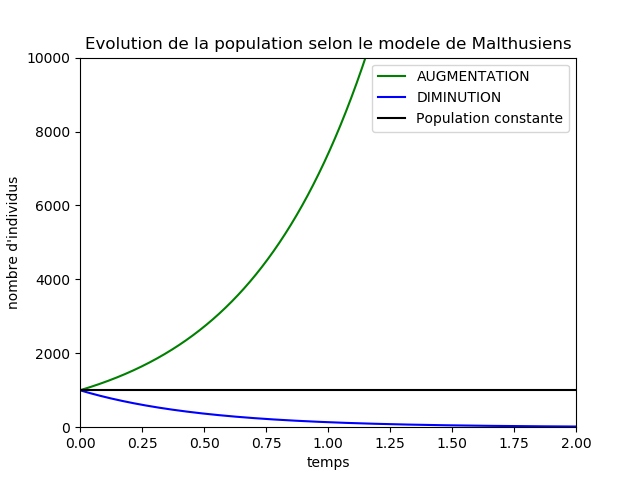
\includegraphics[scale=0.5]{images/Malthus.png}
    \captionsetup{type=figure}\caption{Évolution d'une population selon le modèle de Malthus}
    \label{fig:Malthus}
\end{minipage}
\hfill
\begin{minipage}[c]{.46\linewidth}
    \centering
    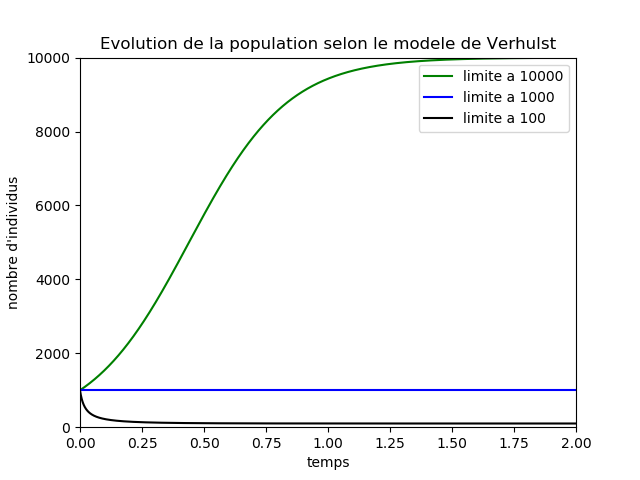
\includegraphics[scale=0.5]{images/Verhulst.png}
    \captionsetup{type=figure}\caption{Évolution d'une population selon le modèle de Verhulst}
    \label{fig:Verhulst}
\end{minipage}
\vspace{4.00mm}

\subsection{Modèle de Lotka-Volterra}
Les deux premiers modèles étudient l'évolution de la population sans prendre en compte les interactions entre les différentes espèces. Le modèle de Lotka-Volterra, modélise les interactions entre une population de proies, notée $N(t)$, et une population de prédateurs, notée $P(t)$, selon les deux équations différentielles suivantes :

\begin{align}
    \frac{dN(t)}{dt} &=  N(t) (a - bP(t)) \\
    \frac{dP(t)}{dt} &=  P(t) (cN(t) - d)
\end{align}

Ainsi, les proies se reproduisent indépendamment des prédateurs. Cependant, leur taux de mortalité est directement relié au nombre de prédateurs. De même, le taux de reproduction des prédateurs dépend des proies rencontrées, mais leur taux de mortalité est indépendant des proies. \\
\begin{minipage}[c]{.46\linewidth}
    \centering
    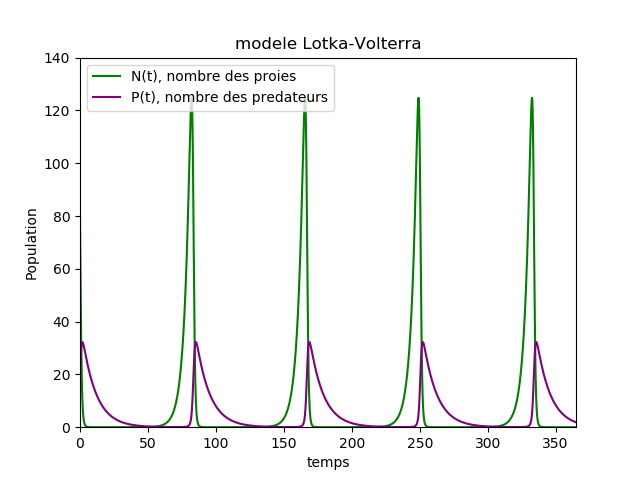
\includegraphics[width=\linewidth]{images/Lotka_Volterra.png}
    \captionsetup{type=figure}\caption{Évolution d'une population selon le modèle de Lotka\_Volterra}
    \label{fig:Lotka_Volterra}
\end{minipage}
\begin{minipage}[c]{.46\linewidth}
    \centering
    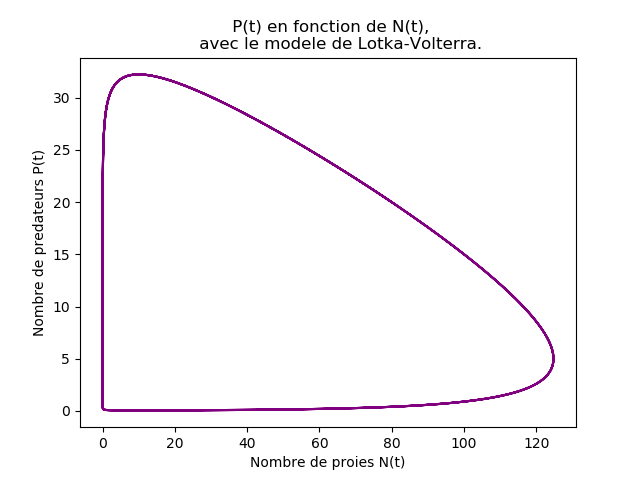
\includegraphics[width=\linewidth]{images/Lotka_Volterra_Pt_Nt.png}
    \captionsetup{type=figure}\caption{Évolution du nombre de prédateurs en fonction du nombre de proies.}
    \label{fig:Nt_Pt}
\end{minipage}
\hfill
\vspace{4.00mm}



D'après la Figure \ref{fig:Lotka_Volterra}, l'évolution des deux espèces est périodique et dépendante. En effet, le nombre de prédateurs augmente rapidement lorsqu'ils sont peu nombreux par rapport au nombre de proies. Par conséquent, le nombre de proies diminue entraînant par la suite une diminution du nombre de prédateurs. Enfin, le nombre de proies ré-augmente du fait qu'il y ait moins de prédateurs, et ainsi de suite.  

La Figure \ref{fig:Nt_Pt} représente le cycle de proie-prédateurs avec 80 proies et 20 prédateurs initialement. Cela correspond au nombre de prédateur en fonction du nombre de proies au cours du temps. On peut constater que l'évolution des 2 populations est cyclique donc infinie : c'est le modèle de cohabitation des espèces, les 2 espèces cohabitent ensemble sans ne jamais s'éteindre. Nous pouvons noter également que la Figure \ref{fig:Nt_Pt} représente $P(t)$ en fonction de $N(t)$ lorsque ces deux fonctions sont des solutions non constantes de l'équation différentielle. D'ailleurs, il existe deux solutions constantes :

\begin{align}
    N(t) &= 0, P(t)=0  \\
    N(t) &= \frac{d}{c}, P(t)=\frac{a}{b}
\end{align}

\begin{minipage}[c]{.46\linewidth}
    \centering
    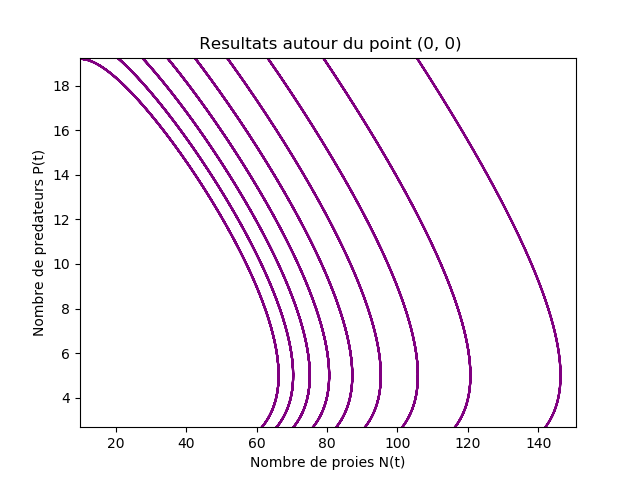
\includegraphics[width=\linewidth]{images/zoom.png}
    \captionsetup{type=figure}\caption{Comportement local au point (0, 0)}
    \label{fig:zoom}
\end{minipage}
\hfill
\begin{minipage}[c]{.46\linewidth}
    \centering
    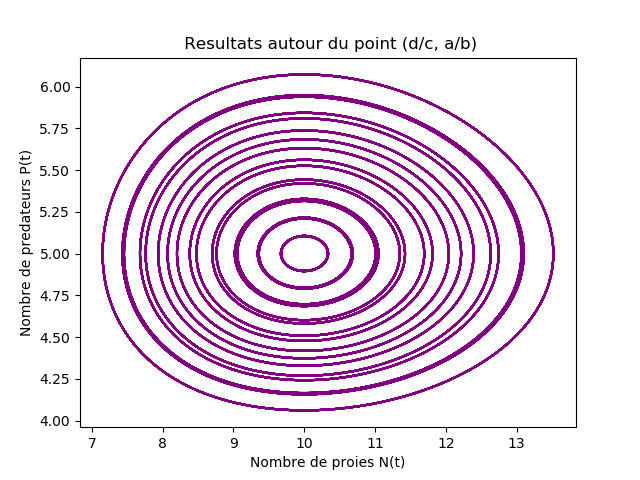
\includegraphics[width=\linewidth]{images/singulier.png}
    \captionsetup{type=figure}\caption{Comportement local au point (d/c, a/b)}
    \label{fig:singulier}
\end{minipage}
\vspace{4.00mm}

Les deux Figures \ref{fig:zoom} et \ref{fig:singulier} montrent que les solutions autour d'un point non singulier, ou bien autour du point $(0,0)$, sont sous la forme d'arcs qui entourent le point. Cependant, les solutions autour du point $(d/c, a/b)$ sont sous la forme de cercles qui entourent le point.
